\subsection{Nanodevices, photonics, and engineered interfaces -- study additions}
\label{study-nano}
\textit{AI-assisted editorial study additions: original explanations and illustrations, not verbatim historical writing nor a transcript. Calendar topics organize this conceptual review; they do not certify course completion, cleanroom training, or experimental competence.}

\subsubsection{From energy bands to a p--n junction}
Closely spaced electronic states in a solid form bands. A semiconductor has a gap between valence and conduction bands; carrier populations depend on temperature, doping, and the Fermi level. Electrons and holes both contribute to transport, with different mobilities and scattering mechanisms. Drift responds to electric field, while diffusion responds to concentration gradients. Equilibrium can have both processes present with zero net current.

When p and n regions form a junction, \textbf{mobile electrons and holes diffuse and recombine near the interface}. The remaining ionized acceptors and donors are bound in the lattice: ordinary depletion is not caused by dopant migration. Negative fixed charge lies on the depleted p side and positive fixed charge on the depleted n side. Their electric field opposes further diffusion. At equilibrium the Fermi level is spatially constant, while band edges bend with electrostatic potential.

For a one-dimensional abrupt junction with uniform doping, the depletion approximation neglects mobile charge inside the space-charge region. Charge balance gives $N_Ax_p=N_Dx_n$. With forward applied voltage $V_A$ and dielectric permittivity $\epsilon$,
\begin{equation}
W=x_p+x_n=\sqrt{\frac{2\epsilon}{q}\left(\frac1{N_A}+\frac1{N_D}\right)(V_{bi}-V_A)}.
\label{study-nano-depletion}
\end{equation}
This approximation excludes breakdown, strong injection, and atomically abrupt behaviour beyond the continuum model. Reverse bias broadens depletion; forward bias reduces the barrier and changes carrier injection. The ideal diode law is therefore a transport result with restrictive assumptions, not simply Ohm's law with a varying resistor.
\begin{figure}[htbp]
\centering
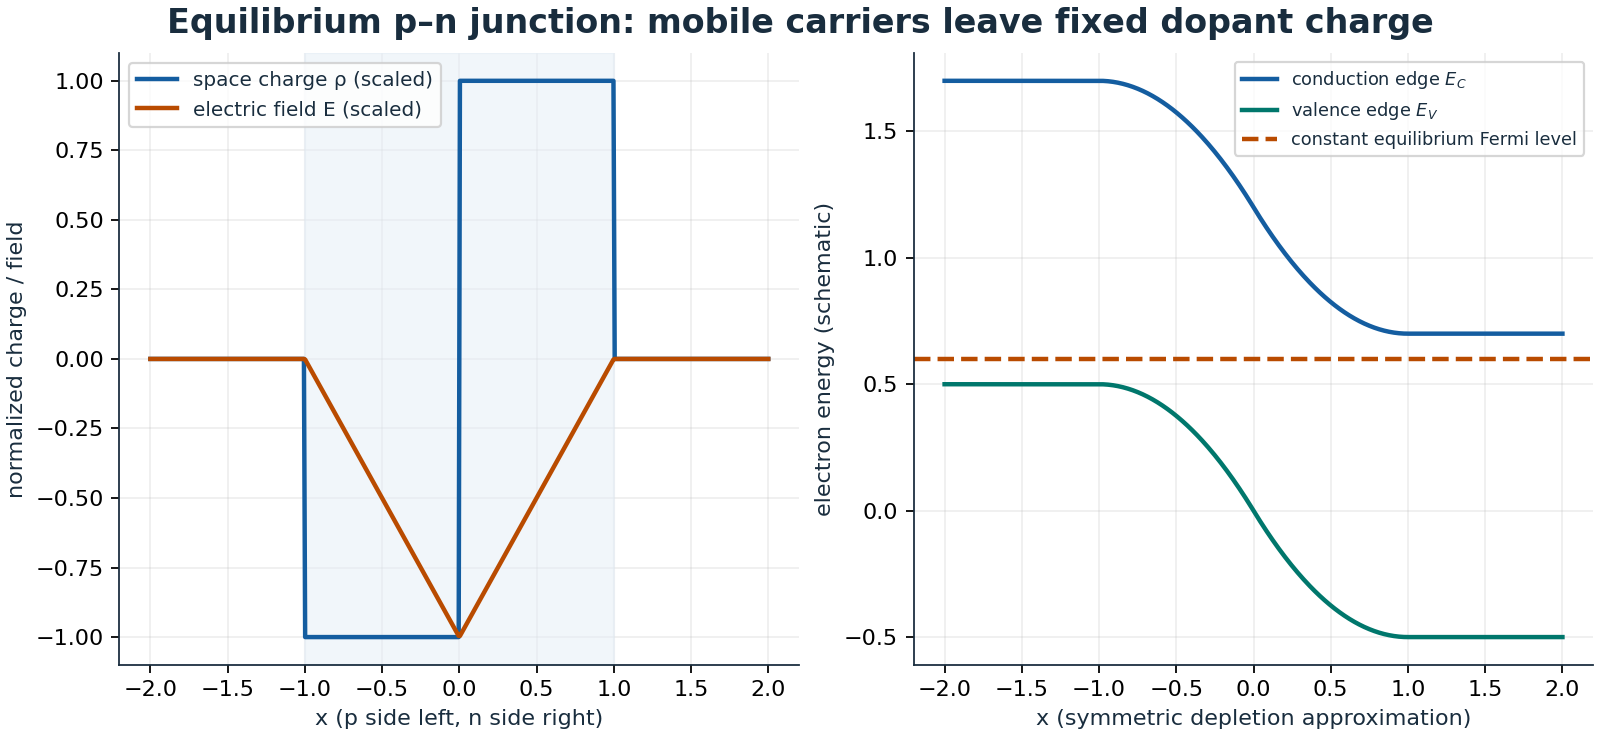
\includegraphics[width=0.95\linewidth]{tex_images/mental_map/study/nano_junction.png}
\caption{Symmetrically doped equilibrium junction in the depletion approximation. Charge and field share normalized axes but different physical units; band edges bend oppositely to electrostatic potential. Fixed dopants do not migrate in this model.}
\end{figure}

\subsubsection{MOS electrostatics and fabrication concepts}
A metal--oxide--semiconductor gate changes surface potential capacitively. Depending on bias and substrate type, the surface accumulates majority carriers, depletes, or inverts. In an n-channel MOSFET on a p-type body, positive gate bias can create an electron inversion channel linking source and drain. Threshold is a model-dependent transition marker, not an infinitely sharp switch. Subthreshold conduction, interface traps, oxide leakage, body bias, and short-channel fields matter in real devices.

The ideal long-channel strong-inversion model gives $I_D=\mu C_{ox}(W/L)[(V_{GS}-V_{th})V_{DS}-V_{DS}^2/2]$ below pinch-off, followed by approximate saturation. Saturation means weak drain-voltage dependence within the model, not a maximum safe current. Small-signal transconductance is a local derivative at a bias point and should not be extrapolated across the full characteristic.
\begin{figure}[htbp]
\centering
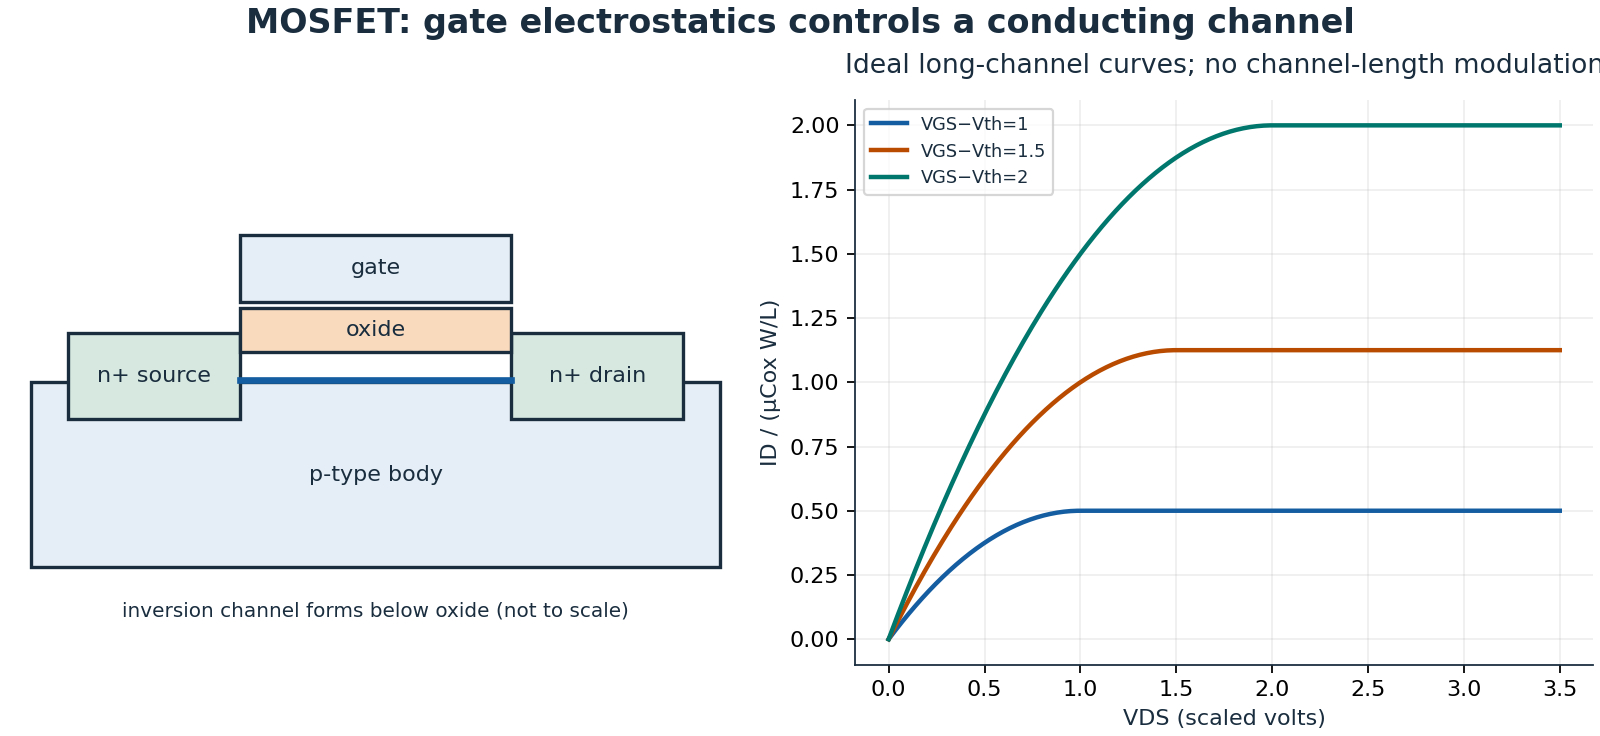
\includegraphics[width=0.95\linewidth]{tex_images/mental_map/study/nano_mosfet.png}
\caption{Schematic n-channel cross-section and ideal normalized long-channel output curves. Layer dimensions are not to scale; channel-length modulation, leakage, velocity saturation, and heating are deliberately omitted.}
\end{figure}

Fabrication conceptually combines substrate selection, film formation, pattern definition, selective material removal, doping, and contacts. Lithography defines where later operations act; deposition and etching alter material geometry. Alignment, selectivity, roughness, stress, contamination, thermal budget, yield, and metrology interact. Top-down patterning and bottom-up self-assembly solve different constraints and may be combined. These principles do not specify chemicals, temperatures, doses, operating sequences, or instructions for cleanroom equipment. A simulated ideal cross-section is not a validated fabrication process.

\subsubsection{Photonics and confinement}
Refractive-index contrast confines guided fields, with evanescent tails extending into cladding. Modes satisfy Maxwell equations and boundary conditions; a ray sketch alone cannot determine nanoscale confinement. Dispersion separates phase and group velocities. Absorption, scattering, bending, and imperfect coupling contribute to loss. Photodetectors convert absorbed photons to electrical signals, while LEDs and lasers require carrier injection and radiative transitions; a laser additionally needs gain overcoming loss and appropriate optical feedback.

Resonators store energy over multiple round trips. A narrower linewidth can improve selectivity but reduce bandwidth and increase sensitivity to drift. High quality factor does not by itself imply efficient coupling or a low-noise measurement. Interference depends on phase coherence, and nanostructures can alter optical density of states without guaranteeing higher external efficiency.
\begin{figure}[htbp]
\centering
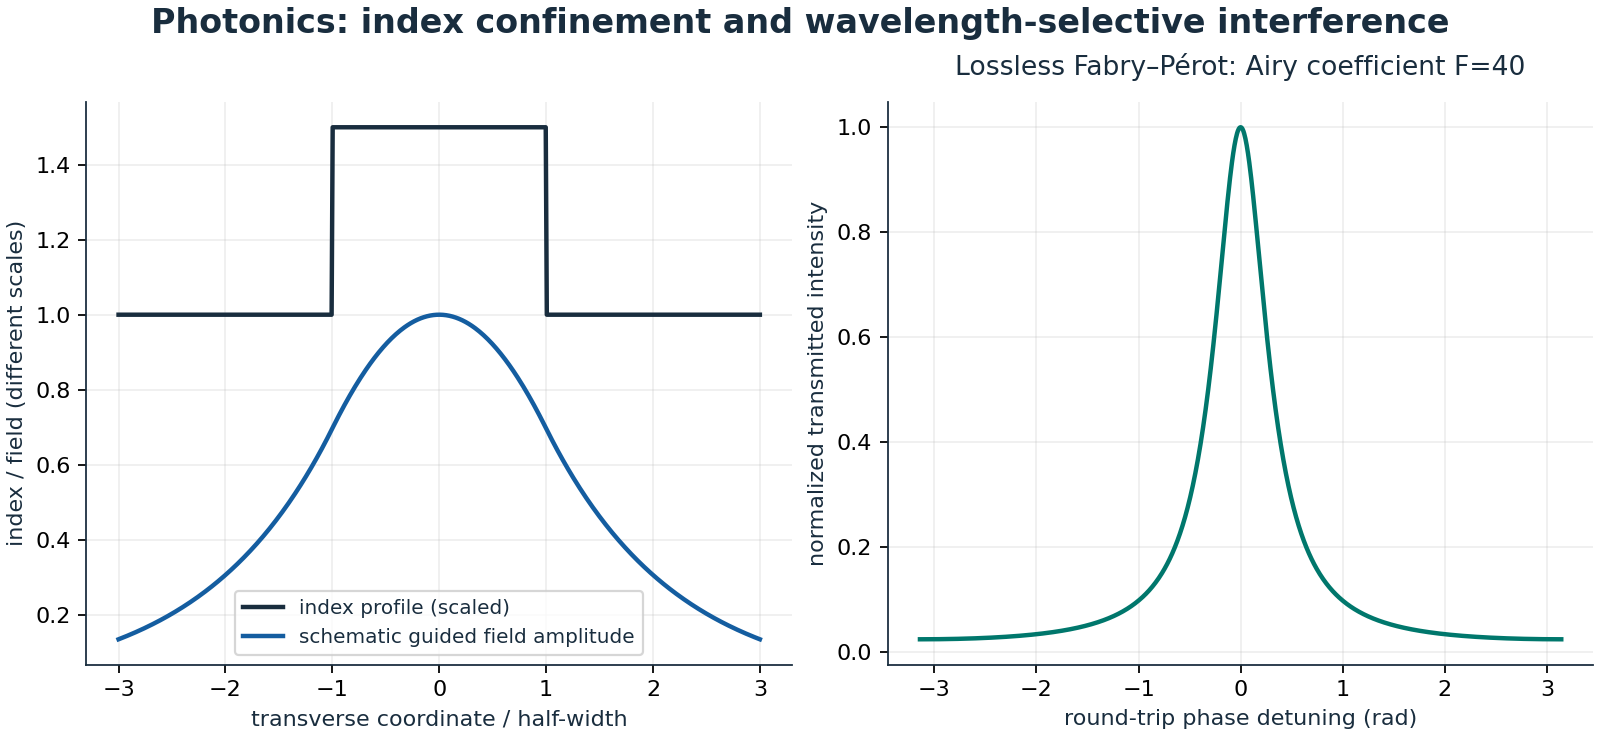
\includegraphics[width=0.95\linewidth]{tex_images/mental_map/study/nano_photonics.png}
\caption{A schematic guided field with evanescent tails beside a lossless Fabry--P\'erot transmission resonance. The index and field use different vertical scales; the mode sketch is not a solved eigenmode for those displayed index values.}
\end{figure}

\subsubsection{Surfaces and electrochemical energy}
Surface-to-volume ratio scales as inverse size for geometrically similar particles, making interface energy, adsorption, and contamination increasingly important. Contact angle balances interfacial tensions only under the assumptions of the relevant wetting model; roughness and hysteresis complicate interpretation. Langmuir adsorption $\theta=Kp/(1+Kp)$ assumes equivalent sites, monolayer occupancy, and no lateral interactions. A successful fit alone does not prove those microscopic assumptions.

For an electrochemical reaction as written, with $n$ electrons transferred,
\begin{equation}
E=E^\circ-\frac{RT}{nF}\ln Q,\qquad\Delta_rG=-nFE.
\label{study-nano-nernst}
\end{equation}
The Nernst equation gives a reversible equilibrium potential using dimensionless activities. At room temperature, a tenfold change in $Q$ changes potential by about $-59.2/n$ millivolts. Measured operating voltage also includes kinetic overpotentials, ohmic losses, and mass transport. A battery's energy capacity and a capacitor's rapid charge storage are different performance measures. Nanostructuring may shorten transport lengths while increasing undesirable side reactions and reducing packing density.
\begin{figure}[htbp]
\centering
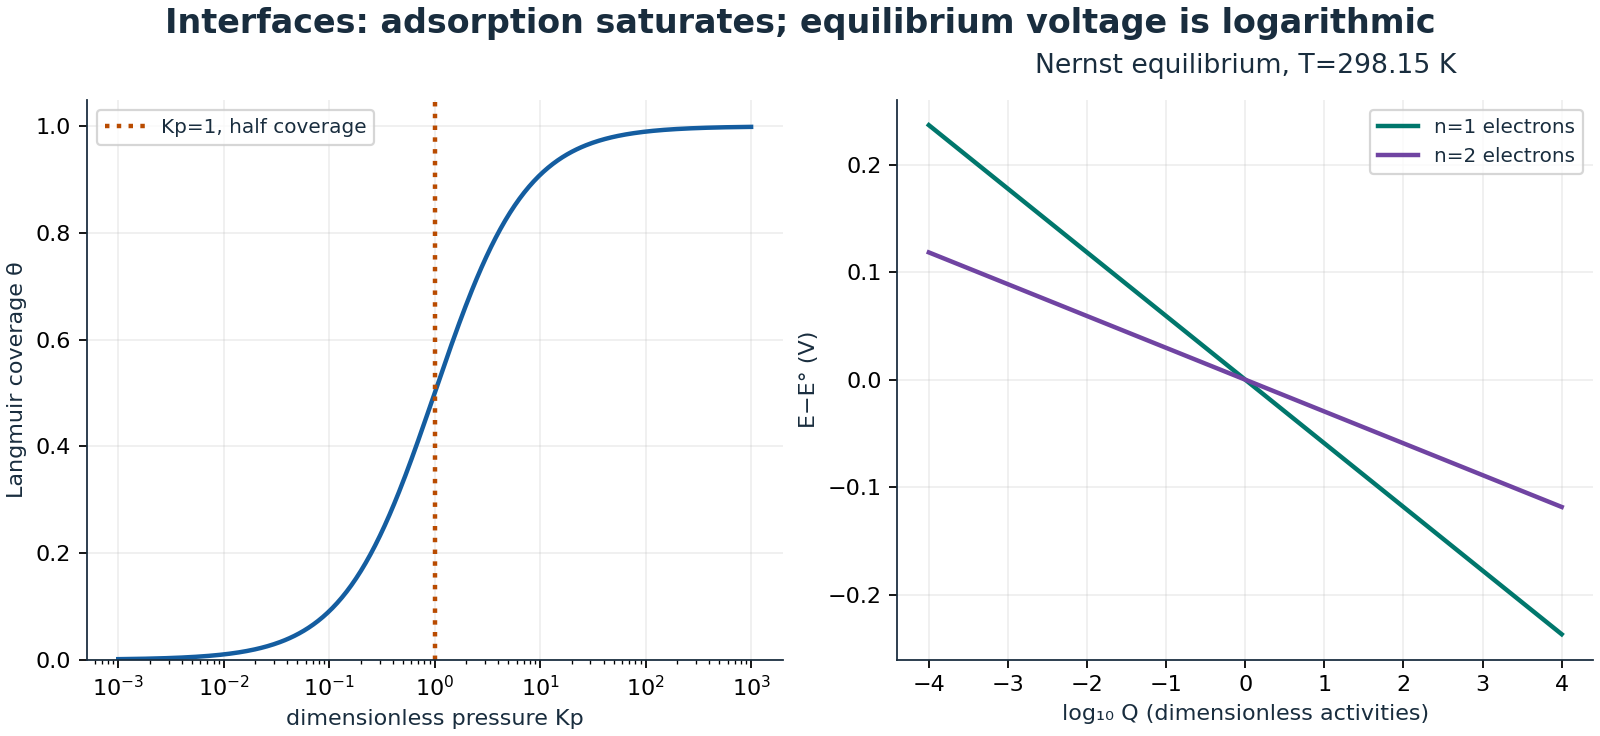
\includegraphics[width=0.95\linewidth]{tex_images/mental_map/study/nano_surfaces.png}
\caption{Ideal independent-site adsorption and Nernst shifts at 298.15 K for one- and two-electron reactions. These equilibrium curves omit electrode kinetics, electrolyte resistance, and transport limitation.}
\end{figure}

\subsubsection{Scope, evidence, and links}
Device equations rely on the physics in Section~\ref{study-physics}; activity and free-energy conventions follow Section~\ref{study-chemistry}; AFM feedback connects characterization to Section~\ref{study-control}. The \href{https://ucalendar.uwaterloo.ca/2223/COURSE/course-NE.html}{Waterloo 2022/23 NE calendar} guides semiconductor, fabrication, photonics, surface, nanoprobing, and electrochemistry scope. It explicitly includes some later offerings, including NE 281 first offered in spring 2024. Such entries cannot substantiate pre-2019 attendance. This review makes no additional course-completion claims. Foundational electrochemical reasoning is also covered in \href{https://openstax.org/details/books/chemistry-2e}{OpenStax Chemistry 2e}.